\section{Cost benefit analysis} % (fold)
\label{sec:cost_benefit_analysis}
To be able to determine the costs and profit of each solution a common measurement is needed. For this case it will be the price of missing a deadline. Since many deadlines are made throughout the planning process across different levels within the organization, it is a difficult point of measurement to be exact about, for a project of the length.

If the project period were longer, the numbers of missed deadlines would be found in meeting minutes from the teams and the budgets, by looking at which deadlines are placed and examining if the deadlines were reached. Based on this, a price for each missed deadline should be found in the consequence of this deadline not being reached. Since this can vary greatly from cheap to expensive consequences a average would be made and used as the overall price for missing a deadline. At this time of the project the price of a missed deadline will be based upon the statements in [\ref{i4q5}] and be 2000 DKK. This is not an accurate estimate by any measure, but can be used in the absence of more precise data. The number of missed deadlines on the level of team leaders is estimated to be 30 per year based on [\ref{i1q13}], as the number of teamleader meetings is estimated to be 10 per year (once every 5 weeks on average).
\\ \\
According to [\ref{i4q7}] the majority of missed deadlines are missed because of a lack of awareness of dependencies between tasks involved. For this reason it is estimated that solution 2 reduces the number of deadlines more than solution 1 as solution 1 does not solve the problem of clarifying dependencies. Based on this, its estimated that solution 1 would reduce the number of deadlines missed by 5 per year, and solution 2 reduce the number of deadlines by 15. For an accurate estimate, it would be necessary to gather data on the causes of each missed deadline, and group these under the problematic categories identified in [\ref{subsec:problems]}. This could be done by performing a survey among the team leaders and arrangers, asking the questions:
\begin{itemize}
\item How often would you estimate that deadlines are missed in the course of a year of planning Musik i Lejet?
\item Describe the main reasons behind deadlines being missed.
\end{itemize}
The second question regarding causes is phrased as an open question, to avoid leading subjects, e.g by listing the reasons revealed by this report. Answers would then have to be categorized, in order to determine which category of reasons, is the most frequent.
\\ \\
Based on the estimates above, the cost benefit analysis found on the next page can be made can be made. Musik i Lejet is a non-profit organization and they have no interest in being able to put money aside each year. Because of this, we have left out the Discounted Cash flow, since this only applies to organizations where a decision about investing or saving is in play.
\newpage
\begin{figure}[h!]
  \centering
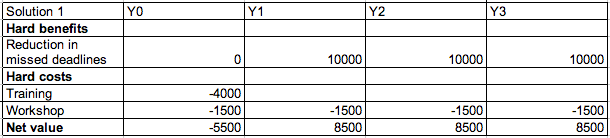
\includegraphics[scale=0.6]{Pictures/cost-benefit1.png}
    \caption{Cost benefit of Podio Work processes (units in DKK)}
\end{figure}
\begin{figure}[h!]
  \centering
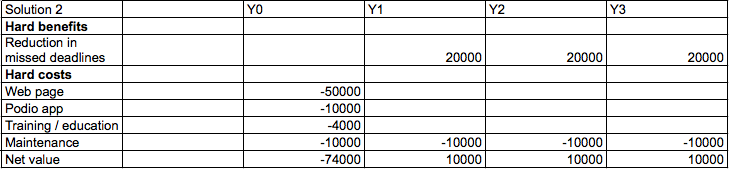
\includegraphics[scale=0.6]{Pictures/cost-benefit2.png}
    \caption{Cost benefit of Podio extension (units in DKK)}
\end{figure}
% section cost_benefit_analysis (end)